%%%%%%%%%%%%%%%%%%%%%%%%%%%%%%%%%%%%%%%%%%%%%%%%%%%%%%%%%%%%%%%%%%%%%%%%%%%%%%%%
%
%   .x~~"*Weu.
%  d8Nu.  9888c
%  88888  98888
%  "***"  9888%
%       ..@8*"
%    ````"8Weu
%   ..    ?8888L
% :@88N   '8888N
% *8888~  '8888F
% '*8"`   9888%
%   `~===*%"`
%
%%%%%%%%%%%%%%%%%%%%%%%%%%%%%%%%%%%%%%%%%%%%%%%%%%%%%%%%%%%%%%%%%%%%%%%%%%%%%%%%

\documentclass[../paper.tex]{subfiles}
\begin{document}

\chapter{Co-Design}
\label{codesign}

Starting with a single Haskell program, the hardware software co-design library is designed with three main tasks in mind: generate C for the software parts, VHDL for the hardware parts, and a combination of C and VHDL for the transmission of data between processing elements. While C and VHDL are different from one another in that one describes sequential software and the other parallel hardware, both languages can be described with an imperative style of programming. As a consequence, the co-design language is based on a monadic representation of imperative programs.

The general idea behind a monad embedding is that one can view an imperative program as a sequence of instructions to be executed on some machine, which looks similar to functions written in a stateful monad. In fact, statements written in a stateful monad can be directly translated into statements in an imperative language. As an example of these similarities, consider the following program for reversing an array in place:

\begin{code}
rev :: SArr Int32 -> Software ()
rev arr = for 0 (len `div` 2) $ \ix -> do
   aix <- getArr arr ix
   ajx <- getArr arr (len - ix - 1)
   setArr arr ix ajx
   setArr arr (len - ix - 1) aix
  where
    len = length arr
\end{code}

Note that \codei{rev} is a software program, as told by its type, but its implementation is not specific to software: for-loops and arrays are part of both C and VHDL. The function could just as well have been implemented in hardware. In fact, a hardware version of \codei{rev} can be defined by swapping its software types with their corresponding hardware types:

\begin{code}
rev :: HArr Int32 -> Hardware ()
\end{code}

The fact that \codei{rev} can be implemented in both software and hardware by simply changing its type does imply that labeling it as either is unnecessarily restrictive. Programs that are constrained by the functionality they require, rather than a specific language, can be described with type classes provided by the co-design language:

\begin{code}
rev :: (Monad m, Arrays m, Control m, Type m Int32) => Arr m Int32 -> m ()
\end{code}

\noindent The now generic \codei{rev} substitutes \codei{SArr} and \codei{HArr} for a \codei{Arr}, the array type associated with monad \codei{m}, and introduces three type classes: \codei{Arrays}, which defines the \codei{Arr} type and its related functions; \codei{Control}, for control flow operations like a for-loop; and \codei{Type}, which ensures a type is representable. Parts of these classes are defined as follows:

\begin{code}
class Monad m => Arrays m where
  type Arr m
  newArr :: Type m a => Exp m Length -> m (Arr m a)
  getArr :: Type m a => Arr m a -> Exp m Index -> m a
  setArr :: Type m a => Arr m a -> Exp m Index -> a -> m ()

class Monad m => Control m where
  for :: (TypeM m a, Integral a) => Exp m a -> Exp m a -> (Exp m a -> m ())
      -> m ()
\end{code}

\noindent where each class lists the functions it provides and in the case of arrays, the type to use with them; \codei{Exp} represents the expression type associated with \codei{m}. The following short-hand for a collection of purely computational operations is defined in order to keep types short:

\begin{code}
type Comp m = (Monad m, References m, Arrays m, Control m)
\end{code}

In addition to the collection of classes in \codei{MonadComp}, there are also classes of operations that only one of the two languages support. The type classes there form a hierarchy with monads at the base. Classes intended for either the software or hardware branches also require the type is an extension of their respective monads. For example, the function for a hardware process is defined by the following type class:

\begin{code}
class HardwareMonad m => Process m where
  process :: m () -> m ()
\end{code}

The co-design language is intended to provide a convenient model of imperative programs and, as was shown in section~\ref{embedded}, also serves as base that extensions like the vector and signal processing languages can be built upon. Furthermore, the ability to write generic programs facilitates design exploration, and while they are not always ideal as hardware description---purely computational instructions does not support, for instance, pipelining---once a layout has been decided, it is easy to fix a program's type to hardware and optimize its implementation.

\section{Imperative Model}
\label{instr}

The co-design language is inspired by the work of Josef and Joel~\cite{BjornBenny} and by the Operational Monad~\cite{Operational}: the program type is deeply embedded in order to capture a computation as an algebraic data type and parameterized on the instructions used in said computations. In addition to instructions, the new program type is also parameterized on a list of other types associated with a program:

\begin{code}
data Program instr fs a
\end{code}

\noindent where the type-level list \codei{fs} could include, for example, the types of subprograms and expressions and a type predicate.

As an instruction's effect will only depend on its interaction with other instructions, they can safely be separated from their sequencing as programs. The task of implementing a program type is therefore equivalent to writing an interpreter for its instructions. One such interpreter, that maps programs to their intended meaning as a monad, is provided by the co-design library:

\begin{code}
interpret :: (Interp i m fs, HFunctor i, Monad m) => Program i fs a -> m a
\end{code}

\codei{interpret} lifts a monadic interpretation of instructions, which may be of varying types, to a monadic interpretation of the whole program. By using different types for the monad \codei{m}, it is possible to implement different ``back ends'' for programs. For example, interpretation in Haskell's \codei{IO} monad creates a way to \emph{run programs}, while interpretation in a code generation monad can be used to make a \emph{compiler}. The interpretation of an instruction set \codei{instr} to the monad \codei{m} is given by \codei{Interp}:

\begin{code}
class Interp instr m fs where
  interp :: instr '(m, fs) a -> m a
\end{code}

\noindent where \codei{'(m, fs)} is type level parameter list of two elements, \codei{m} and \codei{fs}. The second constraint of \codei{interpret}, \codei{HFunctor}, limits instructions to higher-order functors:

\begin{code}
class HFunctor h where
  hfmap :: (forall b . f b -> g b) -> h '(f, fs) a -> h '(g, fs) a
\end{code}

\noindent which lets the interpreter traverse instructions and recursively updated any subprograms they may contain.

Instructions are parameterized on the type of their subprograms to facilitate an compositional definition of them that works for both simple instructions and control instructions, using a technique like Data Types \`{a} La Carte~\cite{DTC}. As both \codei{Interp} and \codei{HFunctor} can be instantiated for a combination of instructions that in turn support their respective class, new instructions can be defined and given an interpretation without worrying about whatever instruction set they are part of. Instructions that can be extended in this way are quite useful to the co-design language, as each computational element usually come with its own set of operations.

As an example of an instruction and how they are interpreted, consider the following datatype that models if-statements:

\begin{code}
data If fs a where
  If :: exp Bool -> prog () -> prog () -> ControlCMD (P3 prog exp pred) ()
\end{code}

\noindent where \codei{P3} is synonym for a type-level list of three arguments---although \codei{pred} is not used by \codei{If}, it is included to keep its type consistent with other instructions that do use it. A program with can now add \codei{If} to its set of instructions like so:

\begin{code}
type MyProgram = Program (Old :+: If) (P2 Exp Pred)
\end{code}

\noindent The program applies itself, \codei{Exp}, and \codei{Pred} as arguments for its instruction set. The \codei{HFunctor} instance for \codei{If} is straightforward:

\begin{code}
instance HFunctor If where
  hfmap f (If c thn els) = If c (f thn) (f els)
\end{code}

If the old instruction set of \codei{MyProgram} supported interpretation in, for instance, the C code generation monad \codei{CGen}, then the added \codei{If} type must support the same interpretation before the instruction stack can be compiled again. Assuming \codei{Exp} can be interpreted in the \codei{CGen} monad, the instance for \codei{If} can be defined as:

\begin{code}
instance Interp If CGen (P2 Exp Pred) where
  interp (If b tru fls) = do
    cc <- compExp b
    addStm [cstm| if ($cc) {$items:tru} else {$items:fls} |]
\end{code}

\noindent where \codei{addStm} adds the quoted C statement to the code generator---quotation is provided by the Haskell package \textit{language-c-quote}.

\codei{interp} is by no means the only interpretation available for programs. For example, the above \codei{If} type has two sub-structures that can be mapped, \codei{prog} and \codei{exp}, and \codei{If} is thus a higher-order \textit{bi-functor}:

\begin{code}
class HFunctor h => HBifunctor h where
  hbimap :: (Functor f, Functor g)
    => (forall b . f b -> g b)
    -> (forall b . i b -> j b)
    -> h '(f, '(i, fs)) a
    -> h '(g, '(j, fs)) a
\end{code}

\noindent This special kind of functor is beneficial in that it enables an interpretation scheme which decouple the interpretation of instructions from that of expressions:

\begin{code}
interpretBi :: (InterpBi instr m fs, HBifunctor instr, Functor m, Monad m)
  => (forall b . exp b -> m b) -> Program instr '(exp, fs) a -> m a
\end{code}

\section{Expressions}
\label{expr}

An embedding based on monads provides a representation of the statements for imperative languages, but most meaningful languages also include a notion of pure expressions. These expressions contain a combination of one or more values, constants, variables, and operators that take two or more expressions. As a small example of such expressions in the co-design language, consider a function for computing the distance between two points in a plane:

\begin{code}
dist :: (SExp Float, SExp Float) -> (SExp Float, SExp Float) -> SExp Float
dist (x1, y1) (x2, y2) = sqrt (dx**2 + dy**2)
  where
    dx = x1 - x2
    dy = y1 - y2
\end{code}

\codei{dist} certainly has the look and feel of a ordinary Haskell expression, but wraps its result \codei{a} in the expression type \codei{exp}. In the co-design language, expressions have a deeply embedded core syntax, and a type of \codei{exp a} is therefore a computation that produces a value of type \codei{a} rather than just a value. The pairs are purely syntactical sugar, as they are not part of the expression syntax and will be removed during interpretation. Also, while \codei{dist} is implemented using \codei{SExp} for software expressions, it could have been defined as a generic expression as well:

\begin{code}
dist :: (Floating (exp a), Num (exp a), Syntax exp a) =>
        (exp a, exp a) -> (exp a, exp a) -> exp a
\end{code}

In addition to the standard numerical and floating point operations, the co-design language also provides a number of higher-order abstractions, like let-bindings:

\begin{code}
class Let exp where
  share :: (Type exp a, Type exp b) => exp a -> (exp a -> exp b) -> exp b
\end{code}

\noindent Such abstractions are one of the hallmarks of functional programming and let users avoid unnecessary detail and mundane operations. At the same time, abstractions can however complicate the compilation processes and make it harder to generate efficient code. To address this problem, the co-design language makes use of two expression types: one with only primitive operations that is easy to compile, and one that includes higher-order features. The idea is then to provide an elaboration from the feature rich expressions to program snippets over primitive expressions:

% Seeing as the feature rich expression type is an extension of the basic one, the two does inevitable share a few primitives and are therefore defined using a technique similar to Data Types \`{a} La Carte---like the instructions from section~\ref{instr}.

\begin{code}
elaborateSExp :: SExp a -> Program SIns (P2 CoreExp SPred) (CoreExp a)
\end{code}

\noindent Wrapping the primitive expressions in programs is necessary to elaborate, for instance, let-bindings, as those are replaced with reference statements.

\codei{elaborateSExp} provides a means to elaborate a single software expression. In order to elaborate an entire program, each instruction must be traversed to find and elaborate any expressions they contain. However, as the result of \codei{elaborateSExp} is monadic, this traversal can be described as interpretation of programs with rich expressions to programs with primitive expressions. This idea is captured by the following function:

\begin{code}
elaborate :: HBifunctor ins1
    => (forall b . exp1 b -> Program ins2 '(exp2, fs) (exp2 b))
    -> Program ins1 '(exp1, fs) a -> Program ins2 '(exp2, fs) a
\end{code}

\noindent Compilation, for instance, can now be defined in two steps: first an elaboration to trim expressions, then an interpretation of the resulting program. This staged approach has a few benefits: it is typed, which rule out many potential errors, and it is easier to write than a complete translation into source code.

\section{Components}

The hardware software co-design language aims to fully describe a modern FPGA, which includes the communication between processing elements. This communication is typically done over an AXI4 interconnect. Full AXI4 offers a range of interconnects that include variable data and address bus widths, high bandwidth burst and cached transfers, and various other transaction features that makes it useful for streaming.

A lighter version of the AXI4 interconnect is offered through AXI4-lite, which is a subset of the full specification that forgoes the streaming features for a simpler communication model that writes and reads data one piece at a time. While a full AXI4 interconnect certainly is useful, implementing one in the co-design language is still future work. An implementation of the AXI4-lite interconnect is however provided:

\begin{code}
axi4lite :: AXIPred a
  => Component a
  -> Component (
          Sig (Bits 32) -- Write address.
       -> Sig (Bits 3)  -- Write channel protection type.
       -> Sig Bit       -- Write address valid.
       -> Sig Bit       -- Write address ready.
       -> Sig (Bits 32) -- Write data.
       -> Sig (Bits 4)  -- Write strobes.
       -> Sig Bit       -- Write valid.
       -> Sig Bit       -- Write ready.
       -> Sig (Bits 2)  -- Write response.
       -> Sig Bit       -- Write response valid.
       -> Sig Bit       -- Response ready.
       -> Sig (Bits 32) -- Read address.
       -> Sig (Bits 3)  -- Protection type.
       -> Sig Bit       -- Read address valid.
       -> Sig Bit       -- Read address ready.
       -> Sig (Bits 32) -- Read data.
       -> Sig (Bits 2)  -- Read response.
       -> Sig Bit       -- Read valid.
       -> Sig Bit       -- Read ready.    
       -> ())
\end{code}

\codei{axi4lite} takes any hardware component of type \codei{a}, assuming \codei{a} can be transmitted over wires, and automatically connects it to an AXI4-lite interconnect. The signals generated by \codei{axi4lite} all follow the AXI4 naming standard, and should as such be recognized by most hardware synthesizers as a valid interconnect. In case the detection does not work, or simply is not supported, it is also possible to add the component manually to a design, as shown in appendix~\ref{}.

Hardware components on the FPGA can interface with each other using port-maps as usual, but an component that is wrapped in an AXI4 interconnect can also be accessed from software with the help of memory-mapped I/O. The general idea is that memory-mapping into a component's physical address causes it to share its address space with the memory of whatever software program is running, that is, the component can be reached by simply reading and writing to pointers into its address. The necessary memory-mapping to connect to a component from software is done by the \codei{mmap}:

\begin{code}
mmap :: Address -> Component a -> Software (Pointer (Soften a))
\end{code}

\noindent Note that \codei{mmap} ``softened'' the component's type by translating its hardware types to their corresponding type in software. A softened pointer can be called from software with a matching set of arguments:

\begin{code}
call :: Pointer a -> Argument a -> Software ()
\end{code}

As an example of offloading a program to hardware and interfacing with it from software, consider the sequential dot product from section~\ref{program} implemented as a hardware program with the following type:

\begin{code}
dotSeq :: HArr Int32 -> HArr Int32 -> Hardware (HExp Int32)
\end{code}

\noindent Types are not first-class values in Haskell, and cannot be inspected by other functions. In order to connect \codei{dotSeq} to an AXI4 interconnect, it must first be given a type signature declaration that is represented using a regular datatype within Haskell, which then can be inspected by other functions. An example of such an signature is given for \codei{dotComp}:

% \noindent While we as designers can read the type of the dot product, other functions cannot. So, before we can hook up the dot-product to an AXI4-lite interconnect and offload it, we need to give it a type signature that can be read by other functions. Seeing as the dot-product takes two arrays as input and then produces an expression as output, we can give it the following signature:

\begin{code}
dotComp :: Component (HArr Int32 -> HArr Int32 -> Signal Int32 -> ())
dotComp = inputArr 3 $ \a -> inputArr 3 $ \b -> outputVal $ dotSeq a b
\end{code}

\noindent which declares a signature of two input arrays, both with a length of three, and a combinatorial output given by \codei{dotSeq}.

To offload \codei{dotSeq} to hardware, it is first wrapped in an AXI4-lite interconnect by calling \codei{axi4lite}, it is then compiled to a VHDL design and synthesized and, lastly, the generated bit stream is loaded onto, for example, an FPGA's programmable logic. During synthesis, the physical address of the design is established. This address can then be accessed from software with the help of \codei{mmap} and \codei{call}:

\begin{code}
program :: Software ()
program = do
  dot <- mmap "0x4C300000" dotComp
  arr <- initArr [1 .. 3]
  brr <- initArr [3 .. 6]
  res <- newRef
  call dot (arr :>> brr :>> res :> nil)
  val <- getRef res
  printf "%d\n" val
\end{code}

\noindent Here, \codei{(:>>)} adds an arrays to an argument list, \codei{(:>)} adds a reference, and \codei{nil} is represents an empty list. The type of \codei{call} ensures that \codei{dot} is called with the correct arguments, after which the result can be read from \codei{res}. The memory mapping only needs to be done once to bring the a pointer to the hardware component into scope, whereas calling an component can be done any number of times.

\section{Vectors}
\label{vectors}

A sequential program in the co-design language makes use of its array type to express array and vector computations with mutable updates. Arrays provide full control over their allocation and assignment, but do so through a low-level and imperative interface. As shown in section~\ref{embedded}, some functions are better expressed in a compositional manner than as a sequential program. For such cases, the vector language provides a useful set of combinators.

Vector computations typically start with a \textit{manifest} vector, that is, a vector that refers directly to an array stored in memory. Vector operations are then applied, where each operation is overloaded to accept any \textit{pully} vector as input and produces another pully vector. Then, once the various vectors have been constructed, they are assembled into a \textit{pushy} vector and written to memory, resulting in a new manifest vector. The names for manifest, pully and pushy vectors draw inspiration from the Pan language~\cite{elliott2003} and push arrays~\cite{claessen2012}, where pushy and pully vectors are methods of computing arrays, rather than elements stored in memory like manifest vectors.

A pully vector consists of a length---the number of elements in the vector---and a function that, given an index in the vector, returns an element. Furthermore, pull vectors are designed in such a way that all operations fuse together without creating any intermediate structures in memory, a property which is often referred to as vector fusion. Pull vectors are represented as:

\begin{code}
data Pull exp a where
  Pull :: exp Length -> (exp Index -> a) -> Pull exp a
\end{code}

Push vectors go in the opposite direction of pull vectors, and provides control over a vectors evaluation to the producers rather than the consumer, that is, pushy vectors have a representation that supports nested writes to memory and fusion of operations. A \codei{Push} vector is represented as:

\begin{code}
data Push m a where
  Push :: Exp m Length -> ((Exp m Index -> a -> m ()) -> m ()) -> Push m a
\end{code}

\noindent A push vector consists of a length, like pull vectors, but its function describes how elements are evaluated rather then how they are fetched. As such, they are parameterized on the monad \codei{m} rather than an expression language; \codei{Exp} is an associated type that refers to the expression type associated with \codei{m}. Push arrays implement efficient concatenation and interleaving, which would otherwise introduce unnecessary conditionals had they been implemented with pull vectors instead.

As an example of vectors, consider the sum of the square of all numbers from zero to $n$:

\begin{code}
squares :: (Num a, Type exp a) => exp a -> exp a
squares n = sum $ map (\x -> x * x) (1 ... n)
\end{code}

\noindent Note that no vector occurs in the function's type, but they are used internally to compute the result: the infix function \codei{(...)} constructs a pully vector with values ranging from one to $n$, to which a mapping is applied that squares each element. The vector is then converted into a push vector by \codei{sum} and summed up into a single value.

Each vector type has a different set of operations associated with it, and these operations are chosen in such a way that each vector type only supports those operations which can be performed efficiently for that type. In many cases, the vector type is guided by the types of the operations involved, and follows the typical pattern of a manifest vector being turned into a pull vector, which turns into a push vector, which is then written to memory and thus turns back into a manifest vector. There are however cases where its preferable to ``skip'' parts of the cycle. For instance, the \codei{squares} function starts with a pull vector rather than a manifest vector.

The functions associated with each kind of vector are overloaded in the kind of vectors they accept: an operation for a pull vector will support the use of any ``pully'' vector type. For instance, the \codei{sum} function used in the above \codei{squares} is defined as follows:

\begin{code}
sum :: (Pully exp vec a, Type exp a, Num a) => vec -> a
sum = fold (+) 0
\end{code}

\section{Signal processing}
\label{signals}

% While the imperative style of programming of the co-design language is already convenient for software realization, section~\ref{embedded} did show that a compositional description can give us a better intuition of what a program consists of. Section~\ref{vectors} addressed this deficiency as its vectors provide a comfortable syntax for composing smaller array functions to form a larger program. For functions that involve a notion of time the signal language is used.

The signal language is based on the concept of signals: possibly infinite sequences of values in some pure expression language, given by the type \codei{Sig}. Conceptually, signals can be thought of as infinite lists. Unlike lists however, a signal is not a first-class value and cannot be nested---it is impossible to construct a signal that produces other signals. Programming with signals is done compositionally, that is, a signal program is a collection of mutually recursive signal functions, each built from repeating values or other signals:

\begin{code}
repeat :: pred a => exp a -> Sig exp pred a

map :: (pred a, pred b) => (exp a -> exp b) ->
  Sig exp pred a -> Sig exp pred b

zipWith :: (pred a, pred b, pred c) => (exp a -> exp b -> exp c) ->
  Sig exp pred a -> Sig exp pred b -> Sig exp pred c
\end{code}

The above signal functions model the similarly named functions in Haskell's base library: \codei{repeat} creates a signal by repeating some value, \codei{map} applies a function to each value of a signal, and \codei{zipWith} joins two signals element-wise using then given function. The idea is to mimic the kind of compositional programming that users normally do in Haskell, or using vectors. Ground types in the expression language are lifted to operate element-wise over signals as well, typically with a type class like \codei{Num}:

\begin{code}
instance (Num (exp a), pred a) => Num (Sig exp pred a) where
  fromInteger = repeat . fromInteger
  (+)         = zipWith (+)
  (-)         = zipWith (-)
  --dotLine
\end{code}

All signal functions shown so far have been combinatorial in nature, in the sense that their output only depends on the current inputs. Sequential functions on the other hand needs to access older values. For these, the signal language provides a unit delay:

\begin{code}
delay :: pred a => exp a -> Sig exp pred a -> Sig exp pred a
\end{code}

\noindent \codei{delay} prepends a value to a signal, delaying its original output by one time instant---the function introduces the notion of a \emph{next time step}, making time enumerable. While \codei{delay} may appear innocent, when combined with feedback it can describe any kind of sequential signal network. For example, a parity checker can be defined as:

\begin{code}
parity :: Sig exp pred Bool -> Sig exp pred Bool
parity inp = out where out = zipWith xor (delay false out) input
\end{code}

As a larger example, we implement a infinite impulse response (IIR) filter, which comprises the second primary type of digital filters used in digital signal processing applications and, unlike FIR filter in section~\ref{embedded}, contains feedback. The IIR filter is typically described and implemented in terms of a difference equation:

\begin{equation}
y_{n} = {1 \over a_{0}} \: \cdot \: \left( \sum_{i=0}^{P} b_{i} \cdot x_{n-i} \: - \: \sum_{j=1}^{Q} a_{j} \cdot y_{n-j} \right)
\end{equation}
\vspace{1mm}

\noindent $P$ and $Q$ are the feed-forward and feedback filter orders and $a_{j}$ and $b_{i}$ are the filter coefficients. Note that $a_{0}$ is used in the outer division and is not part of the feedback sum.

Examining the above equation we can see that the IIR filter loosely consists of two FIR filters, where the second filter has an extra delay and is recursively defined on its output. As such, we can reuse the FIR filter from section~\ref{embed} and define the filter as:

\begin{code}
iir :: (Fractional a, Num (exp a), pred a) => exp a -> [exp a] -> [exp a]
  -> Sig exp pred a -> Sig exp pred a
iir a0 as bs x = y
  where
    y = (1 / repeat a0) * (upper x - lower y)
    upper = fir bs
    lower = fir as . delay 0
\end{code}

A circular definition of \codei{y} in the IIR filter is possible thanks to the \codei{delay} operator, which ensures a productive network as each output only depends on previous input. In general we have that recursively defined signals introduce feedback, while recursion over Haskell values, like lists, can be used to build repeating graphs structures.

This behavior of \codei{delay} implies that we can distinguish values that have and haven't been delayed, which is something that's normally not possible to do in Haskell---being able to observe the sharing of \codei{y} will, by definition, break any referential transparency. In fact, the internals of \codei{delay} makes use of a restricted form of observable sharing~\cite{claessen1999, gill2009}. This allows us to turn signal functions like the above IIR filter into a directed graph. Any sharing is then visible as edges in the graph, connecting the nodes over its operations.

A graph representation of a signal network enables us to check for cycles, order its nodes, and compile it. Regular programs are however a poor target for signal functions, as its type loses any notion of streaming that a function might have had. So, a signal function is instead turned into a co-iterative stream~\cite{caspi1998}, where each stream has an initial state and a transition function from its current state to an output and a new state. The benefit of this approach is that it allows for infinite data types, like streams, to be handled in a strict and efficient way. The streams themselves are however based on programs:

\begin{code}
data Stream instr exp pred a where
  Stream :: Program instr (P2 exp pred) (Program instr (P2 exp pred) a)
    -> Stream instr exp pred a
\end{code}

\noindent A stream's outer program is used to initialize the stream, which results in another program that in turn produces the output values and updates the state.

\end{document}

%%  LocalWords:  pipelining

%%  TODO: put into appendix.

% We show how to synthesize the design manually with the 2015.2 version of Vivado~\cite{feist2012}---the hardware project we're using for our target system requires this specific version. The actual design we're putting onto the FPGA is not important at this point, as the steps outlined below are the same for all designs. 

% Firstly, we create a project for the AXI4 component, and we will use Vivado's tools to give us a template to start from. In particular, we use the ``Create and Package IP'' option under ``Tools'' to launch the creation wizard for a new AXI4 peripheral. Witch we then use to create a AXI4-lite slave, add it to our catalog of IP, and open a editing session for it. Two design files should now exist in our Vivado editor, as show in Figure~\ref{fig:files}.

% \begin{figure}[t]
% 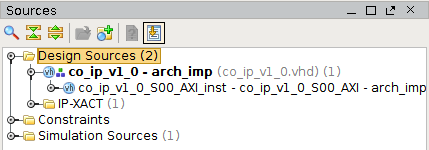
\includegraphics[width=0.4\textwidth]{figures/DesignFiles}
% \centering
% \caption{Design files generated for a AXI4 peripheral.}
% \label{fig:files}
% \end{figure}

% The first file, which is called \codei{co_ip_v1_0} in our example, contains a shell for calling an AXI4-lite slave, and any other we might want to add to the same address space. The second file, called \codei{co_ip_v1_0_S00_AXI_inst}, contains an empty AXI4-lite slave. Its this second file that we substitute with our own design. Note that, after updating the second design, we need to make sure any references from the other design is updated as well. Once that’s done the project can be reviewed and packaged---the review will probably complain that an address port has changed in size, as we always use the full 32 bits rather than a subset, so go ahead and update its size accordingly.

% With our AXI4-lite peripheral saved and packaged, we open up the main project. The system we target is one based on the Zynq board and contains two embedded ARM cores, an FPGA, and possibly a few other accelerators and co-processors, we are however only interested in the first two for now. The block design of our system is given by Figure~\ref{fig:zynq}.

% \begin{figure}[h]
% 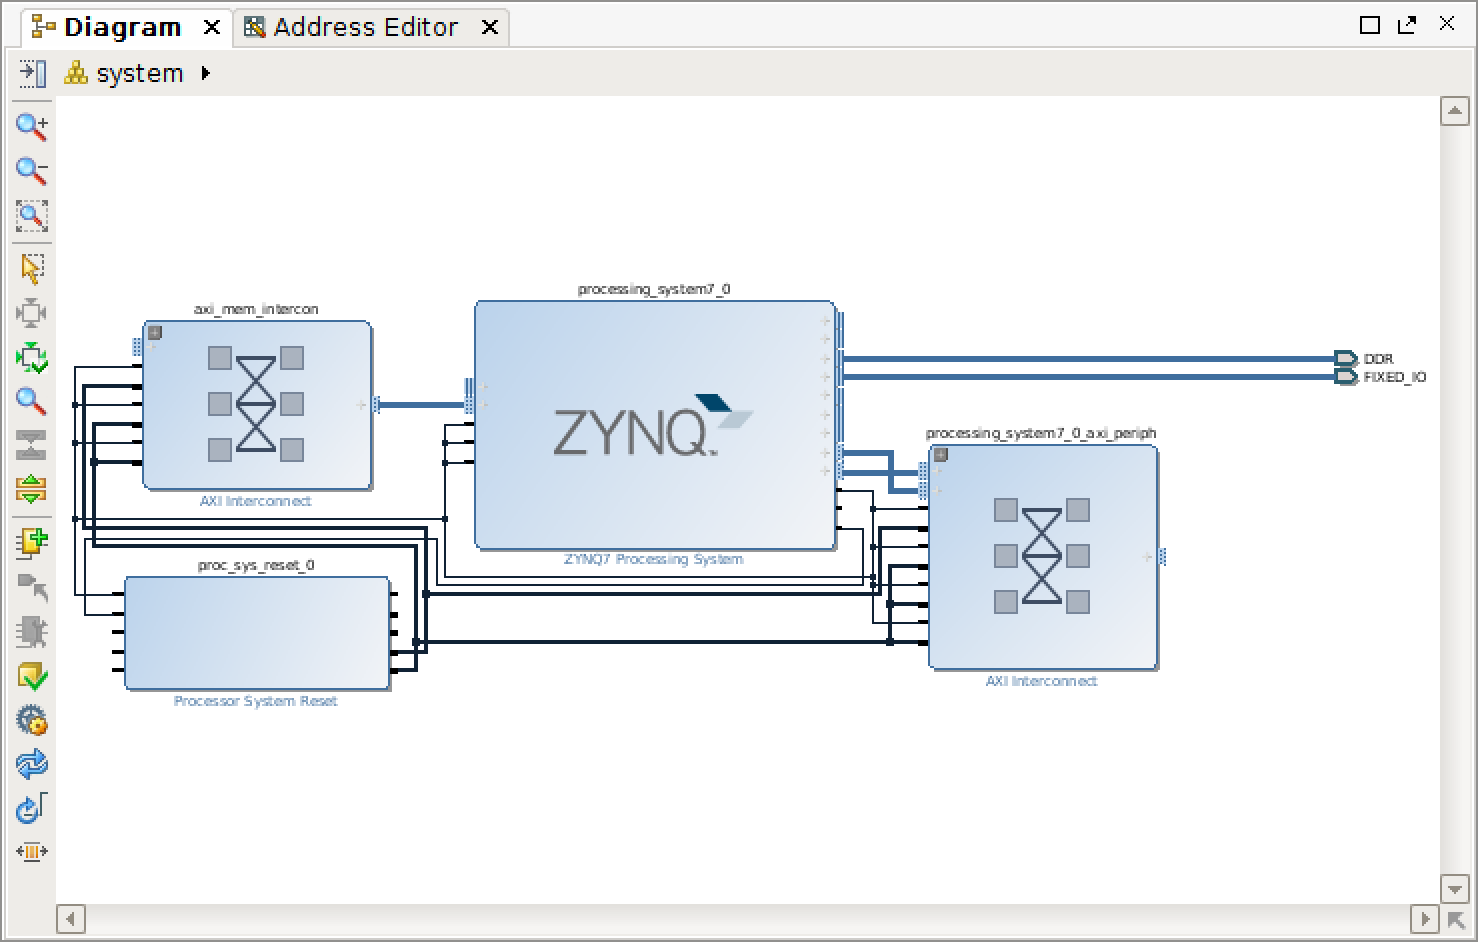
\includegraphics[width=0.4\textwidth]{figures/Zynq}
% \centering
% \caption{Base Zynq project.}
% \label{fig:zynq}
% \end{figure}

% Loading our AXI4-lite peripheral into the main project is straightforward: under the ``IP Settings'' menu, we have the option to locate our newly created project and add it as a repository, from which we can then add its AXI4-lite slave component as an ``IP'' to our main project. With the component added, Vivado can hook it up to our main system automatically through its ``Run Connection Automation'' tool. Finally, we generate a bitstream to put onto the FPGA and get its physical address from the ``Address Editor''. The block design final block design is given by Figure~\ref{fig:system}, and its implementation is given by Figure~\ref{fig:design}.

% \begin{figure}[h]
% 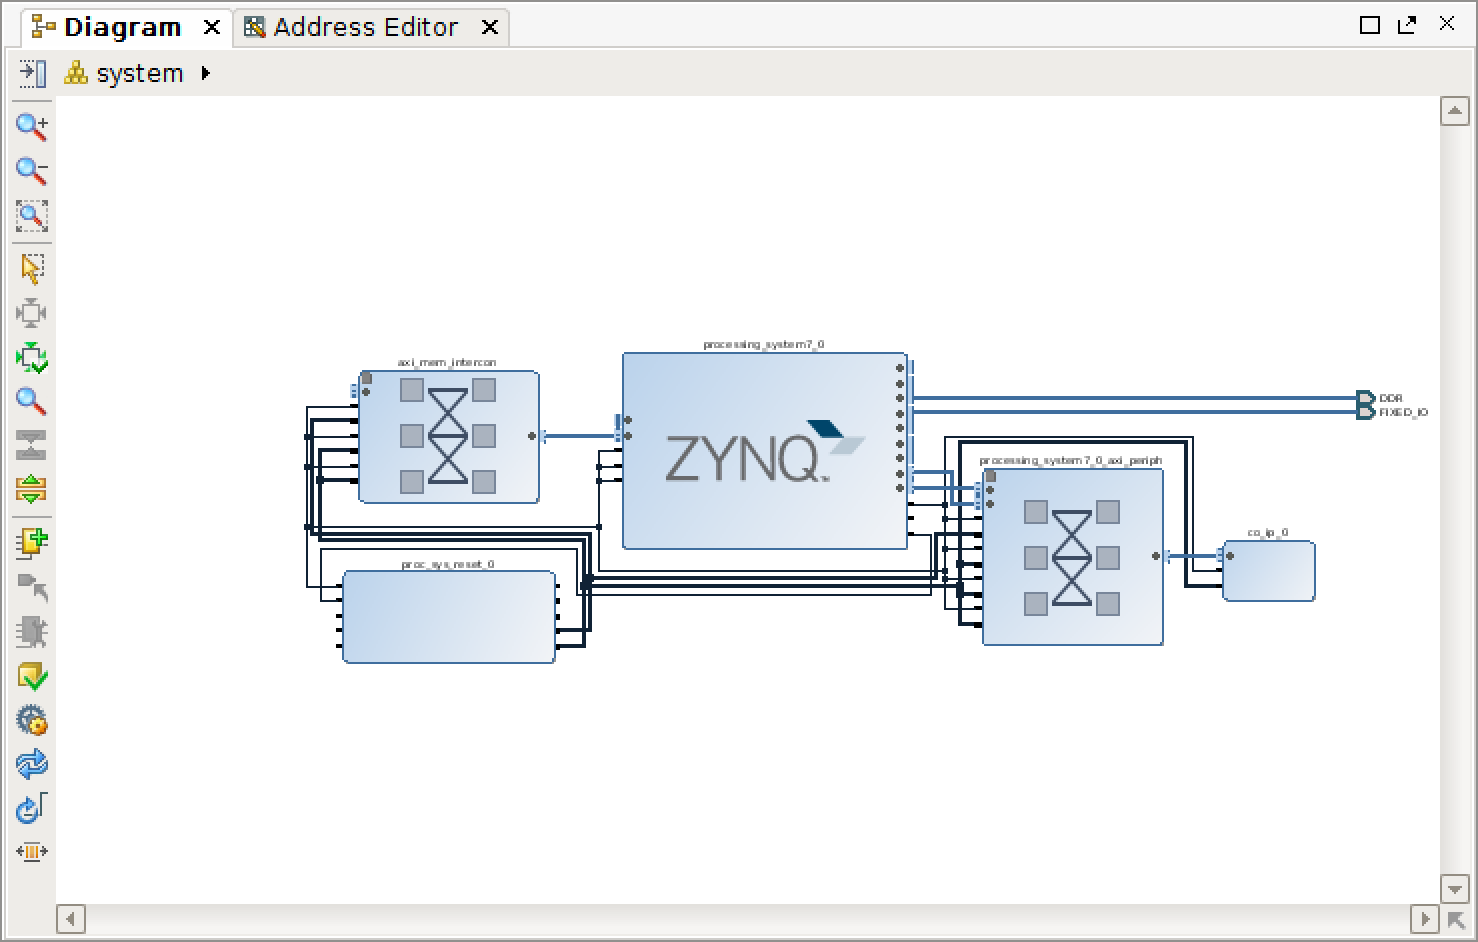
\includegraphics[width=0.4\textwidth]{figures/ZynqSystem}
% \centering
% \caption{Zynq project with AXI4-lite peripheral.}
% \label{fig:system}
% \end{figure}

% \begin{figure}[h]
% 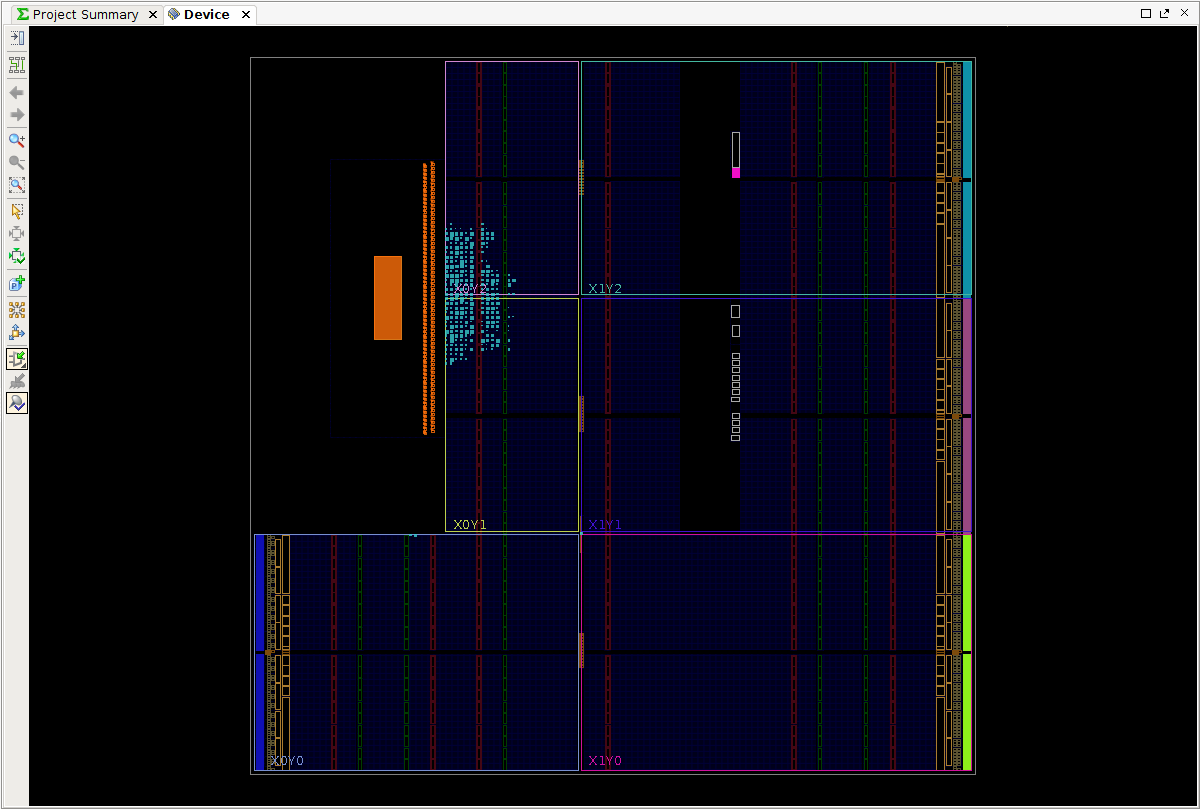
\includegraphics[width=0.4\textwidth]{figures/ZynqDesign}
% \centering
% \caption{Implementation of the project.}
% \label{fig:design}
% \end{figure}

